\documentclass[twoside]{book}

% Packages required by doxygen
\usepackage{fixltx2e}
\usepackage{calc}
\usepackage{doxygen}
\usepackage[export]{adjustbox} % also loads graphicx
\usepackage{graphicx}
\usepackage[utf8]{inputenc}
\usepackage{makeidx}
\usepackage{multicol}
\usepackage{multirow}
\PassOptionsToPackage{warn}{textcomp}
\usepackage{textcomp}
\usepackage[nointegrals]{wasysym}
\usepackage[table]{xcolor}

% Font selection
\usepackage[T1]{fontenc}
\usepackage[scaled=.90]{helvet}
\usepackage{courier}
\usepackage{amssymb}
\usepackage{sectsty}
\renewcommand{\familydefault}{\sfdefault}
\allsectionsfont{%
  \fontseries{bc}\selectfont%
  \color{darkgray}%
}
\renewcommand{\DoxyLabelFont}{%
  \fontseries{bc}\selectfont%
  \color{darkgray}%
}
\newcommand{\+}{\discretionary{\mbox{\scriptsize$\hookleftarrow$}}{}{}}

% Page & text layout
\usepackage{geometry}
\geometry{%
  a4paper,%
  top=2.5cm,%
  bottom=2.5cm,%
  left=2.5cm,%
  right=2.5cm%
}
\tolerance=750
\hfuzz=15pt
\hbadness=750
\setlength{\emergencystretch}{15pt}
\setlength{\parindent}{0cm}
\setlength{\parskip}{3ex plus 2ex minus 2ex}
\makeatletter
\renewcommand{\paragraph}{%
  \@startsection{paragraph}{4}{0ex}{-1.0ex}{1.0ex}{%
    \normalfont\normalsize\bfseries\SS@parafont%
  }%
}
\renewcommand{\subparagraph}{%
  \@startsection{subparagraph}{5}{0ex}{-1.0ex}{1.0ex}{%
    \normalfont\normalsize\bfseries\SS@subparafont%
  }%
}
\makeatother

% Headers & footers
\usepackage{fancyhdr}
\pagestyle{fancyplain}
\fancyhead[LE]{\fancyplain{}{\bfseries\thepage}}
\fancyhead[CE]{\fancyplain{}{}}
\fancyhead[RE]{\fancyplain{}{\bfseries\leftmark}}
\fancyhead[LO]{\fancyplain{}{\bfseries\rightmark}}
\fancyhead[CO]{\fancyplain{}{}}
\fancyhead[RO]{\fancyplain{}{\bfseries\thepage}}
\fancyfoot[LE]{\fancyplain{}{}}
\fancyfoot[CE]{\fancyplain{}{}}
\fancyfoot[RE]{\fancyplain{}{\bfseries\scriptsize Generated by Doxygen }}
\fancyfoot[LO]{\fancyplain{}{\bfseries\scriptsize Generated by Doxygen }}
\fancyfoot[CO]{\fancyplain{}{}}
\fancyfoot[RO]{\fancyplain{}{}}
\renewcommand{\footrulewidth}{0.4pt}
\renewcommand{\chaptermark}[1]{%
  \markboth{#1}{}%
}
\renewcommand{\sectionmark}[1]{%
  \markright{\thesection\ #1}%
}

% Indices & bibliography
\usepackage{natbib}
\usepackage[titles]{tocloft}
\setcounter{tocdepth}{3}
\setcounter{secnumdepth}{5}
\makeindex

% Hyperlinks (required, but should be loaded last)
\usepackage{ifpdf}
\ifpdf
  \usepackage[pdftex,pagebackref=true]{hyperref}
\else
  \usepackage[ps2pdf,pagebackref=true]{hyperref}
\fi
\hypersetup{%
  colorlinks=true,%
  linkcolor=blue,%
  citecolor=blue,%
  unicode%
}

% Custom commands
\newcommand{\clearemptydoublepage}{%
  \newpage{\pagestyle{empty}\cleardoublepage}%
}

\usepackage{caption}
\captionsetup{labelsep=space,justification=centering,font={bf},singlelinecheck=off,skip=4pt,position=top}

%===== C O N T E N T S =====

\begin{document}

% Titlepage & ToC
\hypersetup{pageanchor=false,
             bookmarksnumbered=true,
             pdfencoding=unicode
            }
\pagenumbering{roman}
\begin{titlepage}
\vspace*{7cm}
\begin{center}%
{\Large Usporiadane procesy }\\
\vspace*{1cm}
{\large Generated by Doxygen 1.8.11}\\
\end{center}
\end{titlepage}
\clearemptydoublepage
\tableofcontents
\clearemptydoublepage
\pagenumbering{arabic}
\hypersetup{pageanchor=true}

%--- Begin generated contents ---
\chapter{Class Index}
\section{Class List}
Here are the classes, structs, unions and interfaces with brief descriptions\+:\begin{DoxyCompactList}
\item\contentsline{section}{\hyperlink{struct__App}{\+\_\+\+App} \\*Pseudo-\/objekt specifikacia atributov }{\pageref{struct__App}}{}
\item\contentsline{section}{\hyperlink{struct__Front}{\+\_\+\+Front} \\*Pseudo-\/objekt specifikacia atributov }{\pageref{struct__Front}}{}
\item\contentsline{section}{\hyperlink{struct__Matica}{\+\_\+\+Matica} \\*Pseudo-\/objekt specifikuje atributy }{\pageref{struct__Matica}}{}
\item\contentsline{section}{\hyperlink{struct__Proces}{\+\_\+\+Proces} }{\pageref{struct__Proces}}{}
\end{DoxyCompactList}

\chapter{File Index}
\section{File List}
Here is a list of all documented files with brief descriptions\+:\begin{DoxyCompactList}
\item\contentsline{section}{/home/katka/\+Documents/\+O\+S\+\_\+usporiadane\+Procesy/src/\hyperlink{App_8c}{App.\+c} \\*Modul zodpoveny za beh aplikacie }{\pageref{App_8c}}{}
\item\contentsline{section}{/home/katka/\+Documents/\+O\+S\+\_\+usporiadane\+Procesy/src/\hyperlink{App_8h}{App.\+h} \\*Modul zodpoveny za beh aplikacie }{\pageref{App_8h}}{}
\item\contentsline{section}{/home/katka/\+Documents/\+O\+S\+\_\+usporiadane\+Procesy/src/\hyperlink{Front_8c}{Front.\+c} \\*Modul zodpoveny za riadenie a vytvorenie udajovej strukury front }{\pageref{Front_8c}}{}
\item\contentsline{section}{/home/katka/\+Documents/\+O\+S\+\_\+usporiadane\+Procesy/src/\hyperlink{Front_8h}{Front.\+h} \\*Modul zodpoveny za riadenie a vytvorenie udajovej strukury front }{\pageref{Front_8h}}{}
\item\contentsline{section}{/home/katka/\+Documents/\+O\+S\+\_\+usporiadane\+Procesy/src/\hyperlink{Matica_8c}{Matica.\+c} \\*Modul zodpoveny za riadenie a vytvorenie incidencnej matice }{\pageref{Matica_8c}}{}
\item\contentsline{section}{/home/katka/\+Documents/\+O\+S\+\_\+usporiadane\+Procesy/src/\hyperlink{Matica_8h}{Matica.\+h} \\*Modul zodpoveny za riadenie a vytvorenie incidencnej matice }{\pageref{Matica_8h}}{}
\item\contentsline{section}{/home/katka/\+Documents/\+O\+S\+\_\+usporiadane\+Procesy/src/\hyperlink{Parser_8c}{Parser.\+c} \\*Modul zodpoveny za riadenie a vytvorenie incidencnej matice }{\pageref{Parser_8c}}{}
\item\contentsline{section}{/home/katka/\+Documents/\+O\+S\+\_\+usporiadane\+Procesy/src/\hyperlink{Parser_8h}{Parser.\+h} \\*Modul zodpoveny za riadenie a vytvorenie incidencnej matice }{\pageref{Parser_8h}}{}
\end{DoxyCompactList}

\chapter{Class Documentation}
\hypertarget{struct__App}{}\section{\+\_\+\+App Struct Reference}
\label{struct__App}\index{\+\_\+\+App@{\+\_\+\+App}}


Pseudo-\/objekt specifikacia atributov.  




{\ttfamily \#include $<$App.\+h$>$}

\subsection*{Public Attributes}
\begin{DoxyCompactItemize}
\item 
const char $\ast$ \hyperlink{struct__App_a75b8ceb6c793d2eafac8395c13fc0b0a}{nazov\+\_\+suboru}
\end{DoxyCompactItemize}


\subsection{Detailed Description}
Pseudo-\/objekt specifikacia atributov. 

Reprezentuje instanciu aplikacie 

\subsection{Member Data Documentation}
\index{\+\_\+\+App@{\+\_\+\+App}!nazov\+\_\+suboru@{nazov\+\_\+suboru}}
\index{nazov\+\_\+suboru@{nazov\+\_\+suboru}!\+\_\+\+App@{\+\_\+\+App}}
\subsubsection[{\texorpdfstring{nazov\+\_\+suboru}{nazov_suboru}}]{\setlength{\rightskip}{0pt plus 5cm}const char$\ast$ \+\_\+\+App\+::nazov\+\_\+suboru}\hypertarget{struct__App_a75b8ceb6c793d2eafac8395c13fc0b0a}{}\label{struct__App_a75b8ceb6c793d2eafac8395c13fc0b0a}
Nazov vstupneho suboru s orientovanym grafom. 

The documentation for this struct was generated from the following file\+:\begin{DoxyCompactItemize}
\item 
/home/katka/\+Documents/\+O\+S\+\_\+usporiadane\+Procesy/src/\hyperlink{App_8h}{App.\+h}\end{DoxyCompactItemize}

\hypertarget{struct__Front}{}\section{\+\_\+\+Front Struct Reference}
\label{struct__Front}\index{\+\_\+\+Front@{\+\_\+\+Front}}
\subsection*{Public Attributes}
\begin{DoxyCompactItemize}
\item 
void $\ast$$\ast$ {\bfseries pole}\hypertarget{struct__Front_aaeb70caeedb19e72ba106f621e496942}{}\label{struct__Front_aaeb70caeedb19e72ba106f621e496942}

\item 
size\+\_\+t {\bfseries poc\+\_\+prkov}\hypertarget{struct__Front_a4eadefd147ef83ec0a5f855046ad192a}{}\label{struct__Front_a4eadefd147ef83ec0a5f855046ad192a}

\item 
int {\bfseries akt\+\_\+pozicia\+\_\+pop}\hypertarget{struct__Front_ab755728649fe43c6e3c394ed168387d7}{}\label{struct__Front_ab755728649fe43c6e3c394ed168387d7}

\item 
int {\bfseries akt\+\_\+pozicia\+\_\+push}\hypertarget{struct__Front_a0931c8786584f8671ec4b7c42ba2bdee}{}\label{struct__Front_a0931c8786584f8671ec4b7c42ba2bdee}

\end{DoxyCompactItemize}


The documentation for this struct was generated from the following file\+:\begin{DoxyCompactItemize}
\item 
/home/katka/\+Documents/\+O\+S\+\_\+usporiadane\+Procesy/src/Front.\+h\end{DoxyCompactItemize}

\hypertarget{struct__Matica}{}\section{\+\_\+\+Matica Struct Reference}
\label{struct__Matica}\index{\+\_\+\+Matica@{\+\_\+\+Matica}}
\subsection*{Public Attributes}
\begin{DoxyCompactItemize}
\item 
int $\ast$$\ast$ {\bfseries pole}\hypertarget{struct__Matica_ac3fca0017962cbf096d0e50b54c640b0}{}\label{struct__Matica_ac3fca0017962cbf096d0e50b54c640b0}

\item 
size\+\_\+t {\bfseries velkost\+\_\+strany}\hypertarget{struct__Matica_a089eec293e9332883a0a8963043ae869}{}\label{struct__Matica_a089eec293e9332883a0a8963043ae869}

\end{DoxyCompactItemize}


The documentation for this struct was generated from the following file\+:\begin{DoxyCompactItemize}
\item 
/home/katka/\+Documents/\+O\+S\+\_\+usporiadane\+Procesy/src/Matica.\+h\end{DoxyCompactItemize}

\hypertarget{struct__Proces}{}\section{\+\_\+\+Proces Struct Reference}
\label{struct__Proces}\index{\+\_\+\+Proces@{\+\_\+\+Proces}}


Collaboration diagram for \+\_\+\+Proces\+:\nopagebreak
\begin{figure}[H]
\begin{center}
\leavevmode
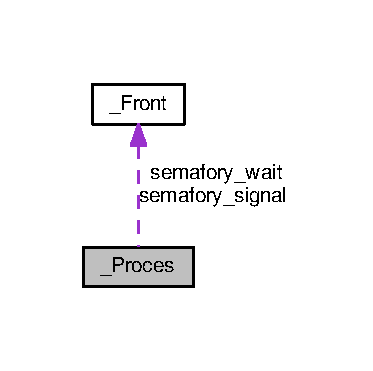
\includegraphics[width=179pt]{struct__Proces__coll__graph}
\end{center}
\end{figure}
\subsection*{Public Attributes}
\begin{DoxyCompactItemize}
\item 
sem\+\_\+t $\ast$ {\bfseries semafor}\hypertarget{struct__Proces_ae861d8129ec67d9e340f035f371d0d1d}{}\label{struct__Proces_ae861d8129ec67d9e340f035f371d0d1d}

\item 
int {\bfseries koeficient}\hypertarget{struct__Proces_adc9eff4877d9e51470d0a9c386b00c40}{}\label{struct__Proces_adc9eff4877d9e51470d0a9c386b00c40}

\item 
\hyperlink{Front_8h_aeda6f9a18e68a801590717ec948afc22}{Front} $\ast$ {\bfseries semafory\+\_\+wait}\hypertarget{struct__Proces_a084d71b0a72065a85df0f51e9b1b3107}{}\label{struct__Proces_a084d71b0a72065a85df0f51e9b1b3107}

\item 
\hyperlink{Front_8h_aeda6f9a18e68a801590717ec948afc22}{Front} $\ast$ {\bfseries semafory\+\_\+signal}\hypertarget{struct__Proces_acb70bd09f8b74c247a3040236a35c2f3}{}\label{struct__Proces_acb70bd09f8b74c247a3040236a35c2f3}

\end{DoxyCompactItemize}


The documentation for this struct was generated from the following file\+:\begin{DoxyCompactItemize}
\item 
/home/katka/\+Documents/\+O\+S\+\_\+usporiadane\+Procesy/src/\hyperlink{App_8c}{App.\+c}\end{DoxyCompactItemize}

\chapter{File Documentation}
\hypertarget{App_8c}{}\section{/home/katka/\+Documents/\+O\+S\+\_\+usporiadane\+Procesy/src/\+App.c File Reference}
\label{App_8c}\index{/home/katka/\+Documents/\+O\+S\+\_\+usporiadane\+Procesy/src/\+App.\+c@{/home/katka/\+Documents/\+O\+S\+\_\+usporiadane\+Procesy/src/\+App.\+c}}


Modul zodpoveny za beh aplikacie.  


{\ttfamily \#include $<$stdio.\+h$>$}\\*
{\ttfamily \#include $<$errno.\+h$>$}\\*
{\ttfamily \#include $<$unistd.\+h$>$}\\*
{\ttfamily \#include $<$stdlib.\+h$>$}\\*
{\ttfamily \#include $<$string.\+h$>$}\\*
{\ttfamily \#include $<$sys/types.\+h$>$}\\*
{\ttfamily \#include $<$fcntl.\+h$>$}\\*
{\ttfamily \#include $<$sys/stat.\+h$>$}\\*
{\ttfamily \#include $<$sys/ipc.\+h$>$}\\*
{\ttfamily \#include $<$sys/shm.\+h$>$}\\*
{\ttfamily \#include $<$sys/mman.\+h$>$}\\*
{\ttfamily \#include $<$semaphore.\+h$>$}\\*
{\ttfamily \#include $<$sys/wait.\+h$>$}\\*
{\ttfamily \#include \char`\"{}Parser.\+h\char`\"{}}\\*
{\ttfamily \#include \char`\"{}App.\+h\char`\"{}}\\*
{\ttfamily \#include \char`\"{}Front.\+h\char`\"{}}\\*
{\ttfamily \#include \char`\"{}Matica.\+h\char`\"{}}\\*
Include dependency graph for App.\+c\+:
\nopagebreak
\begin{figure}[H]
\begin{center}
\leavevmode
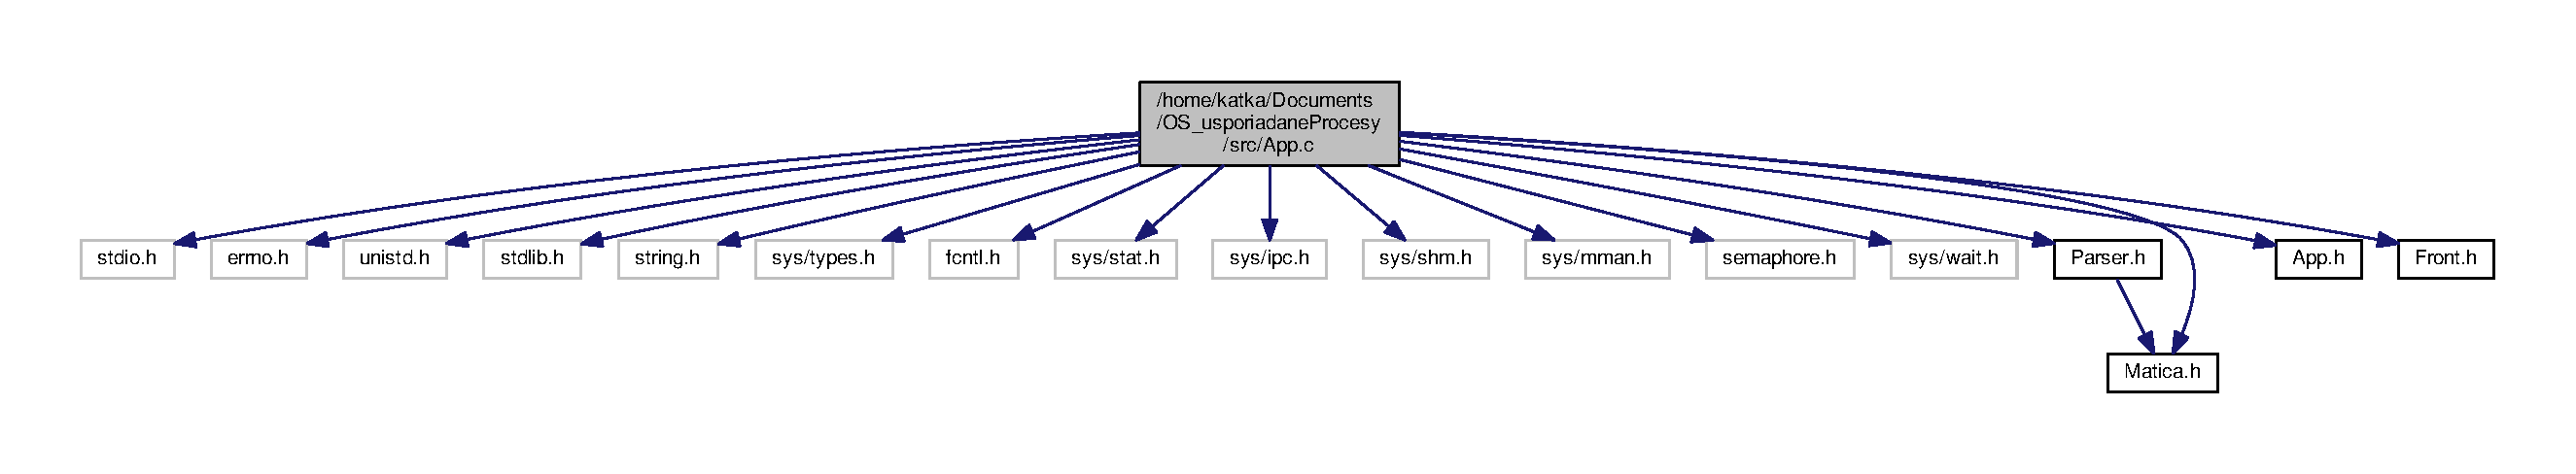
\includegraphics[width=350pt]{App_8c__incl}
\end{center}
\end{figure}
\subsection*{Classes}
\begin{DoxyCompactItemize}
\item 
struct \hyperlink{struct__Proces}{\+\_\+\+Proces}
\end{DoxyCompactItemize}
\subsection*{Macros}
\begin{DoxyCompactItemize}
\item 
\#define {\bfseries \+\_\+\+G\+N\+U\+\_\+\+S\+O\+U\+R\+CE}\hypertarget{App_8c_a369266c24eacffb87046522897a570d5}{}\label{App_8c_a369266c24eacffb87046522897a570d5}

\item 
\#define {\bfseries P\+A\+M\+A\+T\+\_\+\+V\+E\+L\+K\+O\+ST}~4\hypertarget{App_8c_a34b7c9b81912f2424802a302770daa28}{}\label{App_8c_a34b7c9b81912f2424802a302770daa28}

\item 
\#define {\bfseries Z\+D\+\_\+\+P\+A\+M\+A\+T\+\_\+\+K\+L\+UC}~292929\hypertarget{App_8c_a257c4dc7d9729c3bc5e1fd1d2cb734a9}{}\label{App_8c_a257c4dc7d9729c3bc5e1fd1d2cb734a9}

\end{DoxyCompactItemize}
\subsection*{Typedefs}
\begin{DoxyCompactItemize}
\item 
typedef struct \hyperlink{struct__Proces}{\+\_\+\+Proces} {\bfseries Proces}\hypertarget{App_8c_a26e9b69d50adacb680805ff89ce5854c}{}\label{App_8c_a26e9b69d50adacb680805ff89ce5854c}

\end{DoxyCompactItemize}
\subsection*{Functions}
\begin{DoxyCompactItemize}
\item 
\hyperlink{App_8h_a2d680e4981162fefe41e66f322ca6086}{App} $\ast$ \hyperlink{App_8c_a7d31f8de14472b087ff0702d57e51681}{up\+\_\+app\+\_\+vytvor} (const char $\ast$nazov\+\_\+suboru)
\begin{DoxyCompactList}\small\item\em Inicializacia aplikacie. \end{DoxyCompactList}\item 
void \hyperlink{App_8c_a86f98cac61be0021e6c9141b6a851c0b}{up\+\_\+app\+\_\+spusti} (\hyperlink{App_8h_a2d680e4981162fefe41e66f322ca6086}{App} $\ast$inst)
\begin{DoxyCompactList}\small\item\em Spustenie instancie aplikacie. \end{DoxyCompactList}\item 
void \hyperlink{App_8c_ac98160b7755b6ea854f87124264028c1}{up\+\_\+app\+\_\+zrus} (\hyperlink{App_8h_a2d680e4981162fefe41e66f322ca6086}{App} $\ast$inst)
\begin{DoxyCompactList}\small\item\em Zrusenie instancie aplikacie. \end{DoxyCompactList}\end{DoxyCompactItemize}


\subsection{Detailed Description}
Modul zodpoveny za beh aplikacie. 

\begin{DoxyAuthor}{Author}
Katarina Pilarcikova $<$\href{mailto:ketrin.pilarcik@gmail.com}{\tt ketrin.\+pilarcik@gmail.\+com} 
\end{DoxyAuthor}
\begin{DoxyDate}{Date}
20 Dec 2016 
\end{DoxyDate}


\subsection{Function Documentation}
\index{App.\+c@{App.\+c}!up\+\_\+app\+\_\+spusti@{up\+\_\+app\+\_\+spusti}}
\index{up\+\_\+app\+\_\+spusti@{up\+\_\+app\+\_\+spusti}!App.\+c@{App.\+c}}
\subsubsection[{\texorpdfstring{up\+\_\+app\+\_\+spusti(\+App $\ast$inst)}{up_app_spusti(App *inst)}}]{\setlength{\rightskip}{0pt plus 5cm}void up\+\_\+app\+\_\+spusti (
\begin{DoxyParamCaption}
\item[{{\bf App} $\ast$}]{inst}
\end{DoxyParamCaption}
)}\hypertarget{App_8c_a86f98cac61be0021e6c9141b6a851c0b}{}\label{App_8c_a86f98cac61be0021e6c9141b6a851c0b}


Spustenie instancie aplikacie. 


\begin{DoxyParams}{Parameters}
{\em inst} & Smernik na aplikaciu, kt. pozadujeme spustit. \\
\hline
\end{DoxyParams}
\index{App.\+c@{App.\+c}!up\+\_\+app\+\_\+vytvor@{up\+\_\+app\+\_\+vytvor}}
\index{up\+\_\+app\+\_\+vytvor@{up\+\_\+app\+\_\+vytvor}!App.\+c@{App.\+c}}
\subsubsection[{\texorpdfstring{up\+\_\+app\+\_\+vytvor(const char $\ast$nazov\+\_\+suboru)}{up_app_vytvor(const char *nazov_suboru)}}]{\setlength{\rightskip}{0pt plus 5cm}{\bf App}$\ast$ up\+\_\+app\+\_\+vytvor (
\begin{DoxyParamCaption}
\item[{const char $\ast$}]{nazov\+\_\+suboru}
\end{DoxyParamCaption}
)}\hypertarget{App_8c_a7d31f8de14472b087ff0702d57e51681}{}\label{App_8c_a7d31f8de14472b087ff0702d57e51681}


Inicializacia aplikacie. 


\begin{DoxyParams}{Parameters}
{\em nazov\+\_\+suboru} & Nazov vstupneho suboru s orientovanym grafom. \\
\hline
\end{DoxyParams}
\begin{DoxyReturn}{Returns}
Instancia matice. 
\end{DoxyReturn}
\index{App.\+c@{App.\+c}!up\+\_\+app\+\_\+zrus@{up\+\_\+app\+\_\+zrus}}
\index{up\+\_\+app\+\_\+zrus@{up\+\_\+app\+\_\+zrus}!App.\+c@{App.\+c}}
\subsubsection[{\texorpdfstring{up\+\_\+app\+\_\+zrus(\+App $\ast$inst)}{up_app_zrus(App *inst)}}]{\setlength{\rightskip}{0pt plus 5cm}void up\+\_\+app\+\_\+zrus (
\begin{DoxyParamCaption}
\item[{{\bf App} $\ast$}]{inst}
\end{DoxyParamCaption}
)}\hypertarget{App_8c_ac98160b7755b6ea854f87124264028c1}{}\label{App_8c_ac98160b7755b6ea854f87124264028c1}


Zrusenie instancie aplikacie. 


\begin{DoxyParams}{Parameters}
{\em inst} & Smernik na aplikaciu, kt. pozadujeme zrusit. \\
\hline
\end{DoxyParams}

\hypertarget{App_8h}{}\section{/home/katka/\+Documents/\+O\+S\+\_\+usporiadane\+Procesy/src/\+App.h File Reference}
\label{App_8h}\index{/home/katka/\+Documents/\+O\+S\+\_\+usporiadane\+Procesy/src/\+App.\+h@{/home/katka/\+Documents/\+O\+S\+\_\+usporiadane\+Procesy/src/\+App.\+h}}


Modul zodpoveny za beh aplikacie.  


This graph shows which files directly or indirectly include this file\+:
\nopagebreak
\begin{figure}[H]
\begin{center}
\leavevmode
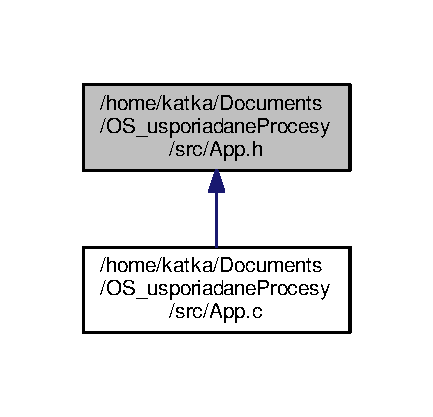
\includegraphics[width=208pt]{App_8h__dep__incl}
\end{center}
\end{figure}
\subsection*{Classes}
\begin{DoxyCompactItemize}
\item 
struct \hyperlink{struct__App}{\+\_\+\+App}
\begin{DoxyCompactList}\small\item\em Pseudo-\/objekt specifikacia atributov. \end{DoxyCompactList}\end{DoxyCompactItemize}
\subsection*{Typedefs}
\begin{DoxyCompactItemize}
\item 
typedef struct \hyperlink{struct__App}{\+\_\+\+App} \hyperlink{App_8h_a2d680e4981162fefe41e66f322ca6086}{App}
\begin{DoxyCompactList}\small\item\em Pseudo-\/objekt specifikacia atributov. \end{DoxyCompactList}\end{DoxyCompactItemize}
\subsection*{Functions}
\begin{DoxyCompactItemize}
\item 
\hyperlink{App_8h_a2d680e4981162fefe41e66f322ca6086}{App} $\ast$ \hyperlink{App_8h_a7d31f8de14472b087ff0702d57e51681}{up\+\_\+app\+\_\+vytvor} (const char $\ast$nazov\+\_\+suboru)
\begin{DoxyCompactList}\small\item\em Inicializacia aplikacie. \end{DoxyCompactList}\item 
void \hyperlink{App_8h_a86f98cac61be0021e6c9141b6a851c0b}{up\+\_\+app\+\_\+spusti} (\hyperlink{App_8h_a2d680e4981162fefe41e66f322ca6086}{App} $\ast$inst)
\begin{DoxyCompactList}\small\item\em Spustenie instancie aplikacie. \end{DoxyCompactList}\item 
void \hyperlink{App_8h_ac98160b7755b6ea854f87124264028c1}{up\+\_\+app\+\_\+zrus} (\hyperlink{App_8h_a2d680e4981162fefe41e66f322ca6086}{App} $\ast$inst)
\begin{DoxyCompactList}\small\item\em Zrusenie instancie aplikacie. \end{DoxyCompactList}\end{DoxyCompactItemize}


\subsection{Detailed Description}
Modul zodpoveny za beh aplikacie. 

\begin{DoxyAuthor}{Author}
Katarina Pilarcikova $<$\href{mailto:ketrin.pilarcik@gmail.com}{\tt ketrin.\+pilarcik@gmail.\+com} 
\end{DoxyAuthor}
\begin{DoxyDate}{Date}
20 Dec 2016 
\end{DoxyDate}


\subsection{Typedef Documentation}
\index{App.\+h@{App.\+h}!App@{App}}
\index{App@{App}!App.\+h@{App.\+h}}
\subsubsection[{\texorpdfstring{App}{App}}]{\setlength{\rightskip}{0pt plus 5cm}typedef struct {\bf \+\_\+\+App}  {\bf App}}\hypertarget{App_8h_a2d680e4981162fefe41e66f322ca6086}{}\label{App_8h_a2d680e4981162fefe41e66f322ca6086}


Pseudo-\/objekt specifikacia atributov. 

Reprezentuje instanciu aplikacie 

\subsection{Function Documentation}
\index{App.\+h@{App.\+h}!up\+\_\+app\+\_\+spusti@{up\+\_\+app\+\_\+spusti}}
\index{up\+\_\+app\+\_\+spusti@{up\+\_\+app\+\_\+spusti}!App.\+h@{App.\+h}}
\subsubsection[{\texorpdfstring{up\+\_\+app\+\_\+spusti(\+App $\ast$inst)}{up_app_spusti(App *inst)}}]{\setlength{\rightskip}{0pt plus 5cm}void up\+\_\+app\+\_\+spusti (
\begin{DoxyParamCaption}
\item[{{\bf App} $\ast$}]{inst}
\end{DoxyParamCaption}
)}\hypertarget{App_8h_a86f98cac61be0021e6c9141b6a851c0b}{}\label{App_8h_a86f98cac61be0021e6c9141b6a851c0b}


Spustenie instancie aplikacie. 


\begin{DoxyParams}{Parameters}
{\em inst} & Smernik na aplikaciu, kt. pozadujeme spustit. \\
\hline
\end{DoxyParams}
\index{App.\+h@{App.\+h}!up\+\_\+app\+\_\+vytvor@{up\+\_\+app\+\_\+vytvor}}
\index{up\+\_\+app\+\_\+vytvor@{up\+\_\+app\+\_\+vytvor}!App.\+h@{App.\+h}}
\subsubsection[{\texorpdfstring{up\+\_\+app\+\_\+vytvor(const char $\ast$nazov\+\_\+suboru)}{up_app_vytvor(const char *nazov_suboru)}}]{\setlength{\rightskip}{0pt plus 5cm}{\bf App}$\ast$ up\+\_\+app\+\_\+vytvor (
\begin{DoxyParamCaption}
\item[{const char $\ast$}]{nazov\+\_\+suboru}
\end{DoxyParamCaption}
)}\hypertarget{App_8h_a7d31f8de14472b087ff0702d57e51681}{}\label{App_8h_a7d31f8de14472b087ff0702d57e51681}


Inicializacia aplikacie. 


\begin{DoxyParams}{Parameters}
{\em nazov\+\_\+suboru} & Nazov vstupneho suboru s orientovanym grafom. \\
\hline
\end{DoxyParams}
\begin{DoxyReturn}{Returns}
Instancia matice. 
\end{DoxyReturn}
\index{App.\+h@{App.\+h}!up\+\_\+app\+\_\+zrus@{up\+\_\+app\+\_\+zrus}}
\index{up\+\_\+app\+\_\+zrus@{up\+\_\+app\+\_\+zrus}!App.\+h@{App.\+h}}
\subsubsection[{\texorpdfstring{up\+\_\+app\+\_\+zrus(\+App $\ast$inst)}{up_app_zrus(App *inst)}}]{\setlength{\rightskip}{0pt plus 5cm}void up\+\_\+app\+\_\+zrus (
\begin{DoxyParamCaption}
\item[{{\bf App} $\ast$}]{inst}
\end{DoxyParamCaption}
)}\hypertarget{App_8h_ac98160b7755b6ea854f87124264028c1}{}\label{App_8h_ac98160b7755b6ea854f87124264028c1}


Zrusenie instancie aplikacie. 


\begin{DoxyParams}{Parameters}
{\em inst} & Smernik na aplikaciu, kt. pozadujeme zrusit. \\
\hline
\end{DoxyParams}

\hypertarget{Front_8c}{}\section{/home/katka/\+Documents/\+O\+S\+\_\+usporiadane\+Procesy/src/\+Front.c File Reference}
\label{Front_8c}\index{/home/katka/\+Documents/\+O\+S\+\_\+usporiadane\+Procesy/src/\+Front.\+c@{/home/katka/\+Documents/\+O\+S\+\_\+usporiadane\+Procesy/src/\+Front.\+c}}


Modul zodpoveny za riadenie a vytvorenie udajovej strukury front.  


{\ttfamily \#include $<$stdlib.\+h$>$}\\*
{\ttfamily \#include \char`\"{}Front.\+h\char`\"{}}\\*
Include dependency graph for Front.\+c\+:
\nopagebreak
\begin{figure}[H]
\begin{center}
\leavevmode
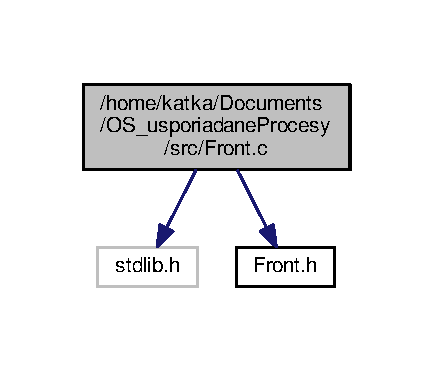
\includegraphics[width=208pt]{Front_8c__incl}
\end{center}
\end{figure}
\subsection*{Macros}
\begin{DoxyCompactItemize}
\item 
\#define {\bfseries P\+O\+V\+O\+D\+N\+A\+\_\+\+V\+E\+L\+K\+O\+ST}~20\hypertarget{Front_8c_ad8c4675683d6f185a8394dfa1bd1ed61}{}\label{Front_8c_ad8c4675683d6f185a8394dfa1bd1ed61}

\end{DoxyCompactItemize}
\subsection*{Functions}
\begin{DoxyCompactItemize}
\item 
\hyperlink{Front_8h_aeda6f9a18e68a801590717ec948afc22}{Front} $\ast$ \hyperlink{Front_8c_a0c58eb9ce291fecc6b520a9a00130de8}{up\+\_\+front\+\_\+vytvor} ()
\begin{DoxyCompactList}\small\item\em Inicializuje front. \end{DoxyCompactList}\item 
void \hyperlink{Front_8c_aa5f6d4ff6866b68e7a82ab188d1e582d}{up\+\_\+front\+\_\+zrus} (\hyperlink{Front_8h_aeda6f9a18e68a801590717ec948afc22}{Front} $\ast$inst)
\begin{DoxyCompactList}\small\item\em Zrusenie frontu. \end{DoxyCompactList}\item 
void \hyperlink{Front_8c_ac80877645f112df1ece1c73b06f79a80}{up\+\_\+front\+\_\+push} (\hyperlink{Front_8h_aeda6f9a18e68a801590717ec948afc22}{Front} $\ast$inst, void $\ast$prvok)
\begin{DoxyCompactList}\small\item\em Pridanie prvku do frontu. \end{DoxyCompactList}\item 
void $\ast$ \hyperlink{Front_8c_ae43c9590e0c795e07914f0965aa917da}{up\+\_\+front\+\_\+pop} (\hyperlink{Front_8h_aeda6f9a18e68a801590717ec948afc22}{Front} $\ast$inst)
\begin{DoxyCompactList}\small\item\em Odobratie prvku z frontu. \end{DoxyCompactList}\item 
void $\ast$ \hyperlink{Front_8c_a23dea24023ffd88914ef499bf0d0c64c}{up\+\_\+front\+\_\+peek} (\hyperlink{Front_8h_aeda6f9a18e68a801590717ec948afc22}{Front} $\ast$inst)
\begin{DoxyCompactList}\small\item\em Spristupnenie prveho prvku na pop. \end{DoxyCompactList}\item 
int \hyperlink{Front_8c_a63e5753b29437dde3926a4b91ca344b1}{up\+\_\+front\+\_\+je\+\_\+prazdny} (\hyperlink{Front_8h_aeda6f9a18e68a801590717ec948afc22}{Front} $\ast$inst)
\begin{DoxyCompactList}\small\item\em Zisti, ci je front prazdny. \end{DoxyCompactList}\item 
size\+\_\+t \hyperlink{Front_8c_a92a54c47c61758146e7c9205f598938f}{up\+\_\+front\+\_\+daj\+\_\+poc\+\_\+prvkov} (\hyperlink{Front_8h_aeda6f9a18e68a801590717ec948afc22}{Front} $\ast$inst)
\begin{DoxyCompactList}\small\item\em Vrati pocet prvkov frontu. \end{DoxyCompactList}\end{DoxyCompactItemize}


\subsection{Detailed Description}
Modul zodpoveny za riadenie a vytvorenie udajovej strukury front. 

\begin{DoxyAuthor}{Author}
Katarina Pilarcikova $<$\href{mailto:ketrin.pilarcik@gmail.com}{\tt ketrin.\+pilarcik@gmail.\+com} 
\end{DoxyAuthor}
\begin{DoxyDate}{Date}
20 Dec 2016 
\end{DoxyDate}


\subsection{Function Documentation}
\index{Front.\+c@{Front.\+c}!up\+\_\+front\+\_\+daj\+\_\+poc\+\_\+prvkov@{up\+\_\+front\+\_\+daj\+\_\+poc\+\_\+prvkov}}
\index{up\+\_\+front\+\_\+daj\+\_\+poc\+\_\+prvkov@{up\+\_\+front\+\_\+daj\+\_\+poc\+\_\+prvkov}!Front.\+c@{Front.\+c}}
\subsubsection[{\texorpdfstring{up\+\_\+front\+\_\+daj\+\_\+poc\+\_\+prvkov(\+Front $\ast$inst)}{up_front_daj_poc_prvkov(Front *inst)}}]{\setlength{\rightskip}{0pt plus 5cm}size\+\_\+t up\+\_\+front\+\_\+daj\+\_\+poc\+\_\+prvkov (
\begin{DoxyParamCaption}
\item[{{\bf Front} $\ast$}]{inst}
\end{DoxyParamCaption}
)}\hypertarget{Front_8c_a92a54c47c61758146e7c9205f598938f}{}\label{Front_8c_a92a54c47c61758146e7c9205f598938f}


Vrati pocet prvkov frontu. 


\begin{DoxyParams}{Parameters}
{\em inst} & Instancia frontu \\
\hline
\end{DoxyParams}
\begin{DoxyReturn}{Returns}
size\+\_\+t Aktualny pocet prvkov frontu. 
\end{DoxyReturn}
\index{Front.\+c@{Front.\+c}!up\+\_\+front\+\_\+je\+\_\+prazdny@{up\+\_\+front\+\_\+je\+\_\+prazdny}}
\index{up\+\_\+front\+\_\+je\+\_\+prazdny@{up\+\_\+front\+\_\+je\+\_\+prazdny}!Front.\+c@{Front.\+c}}
\subsubsection[{\texorpdfstring{up\+\_\+front\+\_\+je\+\_\+prazdny(\+Front $\ast$inst)}{up_front_je_prazdny(Front *inst)}}]{\setlength{\rightskip}{0pt plus 5cm}int up\+\_\+front\+\_\+je\+\_\+prazdny (
\begin{DoxyParamCaption}
\item[{{\bf Front} $\ast$}]{inst}
\end{DoxyParamCaption}
)}\hypertarget{Front_8c_a63e5753b29437dde3926a4b91ca344b1}{}\label{Front_8c_a63e5753b29437dde3926a4b91ca344b1}


Zisti, ci je front prazdny. 


\begin{DoxyParams}{Parameters}
{\em inst} & Instancia frontu \\
\hline
\end{DoxyParams}
\begin{DoxyReturn}{Returns}
0 ak obsahuje prvky, 1 aj je prazdny. 
\end{DoxyReturn}
\index{Front.\+c@{Front.\+c}!up\+\_\+front\+\_\+peek@{up\+\_\+front\+\_\+peek}}
\index{up\+\_\+front\+\_\+peek@{up\+\_\+front\+\_\+peek}!Front.\+c@{Front.\+c}}
\subsubsection[{\texorpdfstring{up\+\_\+front\+\_\+peek(\+Front $\ast$inst)}{up_front_peek(Front *inst)}}]{\setlength{\rightskip}{0pt plus 5cm}void$\ast$ up\+\_\+front\+\_\+peek (
\begin{DoxyParamCaption}
\item[{{\bf Front} $\ast$}]{inst}
\end{DoxyParamCaption}
)}\hypertarget{Front_8c_a23dea24023ffd88914ef499bf0d0c64c}{}\label{Front_8c_a23dea24023ffd88914ef499bf0d0c64c}


Spristupnenie prveho prvku na pop. 


\begin{DoxyParams}{Parameters}
{\em inst} & Instancia frontu z ktoreho zistujeme prvok. \\
\hline
\end{DoxyParams}
\index{Front.\+c@{Front.\+c}!up\+\_\+front\+\_\+pop@{up\+\_\+front\+\_\+pop}}
\index{up\+\_\+front\+\_\+pop@{up\+\_\+front\+\_\+pop}!Front.\+c@{Front.\+c}}
\subsubsection[{\texorpdfstring{up\+\_\+front\+\_\+pop(\+Front $\ast$inst)}{up_front_pop(Front *inst)}}]{\setlength{\rightskip}{0pt plus 5cm}void$\ast$ up\+\_\+front\+\_\+pop (
\begin{DoxyParamCaption}
\item[{{\bf Front} $\ast$}]{inst}
\end{DoxyParamCaption}
)}\hypertarget{Front_8c_ae43c9590e0c795e07914f0965aa917da}{}\label{Front_8c_ae43c9590e0c795e07914f0965aa917da}


Odobratie prvku z frontu. 


\begin{DoxyParams}{Parameters}
{\em inst} & Instancia frontu z ktoreho vyberame. \\
\hline
\end{DoxyParams}
\begin{DoxyReturn}{Returns}
Prvok z prvy vo fronte. 
\end{DoxyReturn}
\index{Front.\+c@{Front.\+c}!up\+\_\+front\+\_\+push@{up\+\_\+front\+\_\+push}}
\index{up\+\_\+front\+\_\+push@{up\+\_\+front\+\_\+push}!Front.\+c@{Front.\+c}}
\subsubsection[{\texorpdfstring{up\+\_\+front\+\_\+push(\+Front $\ast$inst, void $\ast$prvok)}{up_front_push(Front *inst, void *prvok)}}]{\setlength{\rightskip}{0pt plus 5cm}void up\+\_\+front\+\_\+push (
\begin{DoxyParamCaption}
\item[{{\bf Front} $\ast$}]{inst, }
\item[{void $\ast$}]{prvok}
\end{DoxyParamCaption}
)}\hypertarget{Front_8c_ac80877645f112df1ece1c73b06f79a80}{}\label{Front_8c_ac80877645f112df1ece1c73b06f79a80}


Pridanie prvku do frontu. 


\begin{DoxyParams}{Parameters}
{\em inst} & Instancia frontu do ktoreho chceme pridat prvok. \\
\hline
{\em prvok} & Pridavany prvok do frontu. \\
\hline
\end{DoxyParams}
\index{Front.\+c@{Front.\+c}!up\+\_\+front\+\_\+vytvor@{up\+\_\+front\+\_\+vytvor}}
\index{up\+\_\+front\+\_\+vytvor@{up\+\_\+front\+\_\+vytvor}!Front.\+c@{Front.\+c}}
\subsubsection[{\texorpdfstring{up\+\_\+front\+\_\+vytvor()}{up_front_vytvor()}}]{\setlength{\rightskip}{0pt plus 5cm}{\bf Front}$\ast$ up\+\_\+front\+\_\+vytvor (
\begin{DoxyParamCaption}
{}
\end{DoxyParamCaption}
)}\hypertarget{Front_8c_a0c58eb9ce291fecc6b520a9a00130de8}{}\label{Front_8c_a0c58eb9ce291fecc6b520a9a00130de8}


Inicializuje front. 

\begin{DoxyReturn}{Returns}
Pointer na instanciu frontu 
\end{DoxyReturn}
\index{Front.\+c@{Front.\+c}!up\+\_\+front\+\_\+zrus@{up\+\_\+front\+\_\+zrus}}
\index{up\+\_\+front\+\_\+zrus@{up\+\_\+front\+\_\+zrus}!Front.\+c@{Front.\+c}}
\subsubsection[{\texorpdfstring{up\+\_\+front\+\_\+zrus(\+Front $\ast$inst)}{up_front_zrus(Front *inst)}}]{\setlength{\rightskip}{0pt plus 5cm}void up\+\_\+front\+\_\+zrus (
\begin{DoxyParamCaption}
\item[{{\bf Front} $\ast$}]{inst}
\end{DoxyParamCaption}
)}\hypertarget{Front_8c_aa5f6d4ff6866b68e7a82ab188d1e582d}{}\label{Front_8c_aa5f6d4ff6866b68e7a82ab188d1e582d}


Zrusenie frontu. 


\begin{DoxyParams}{Parameters}
{\em inst} & Smernik na instanciu frontu, kt pozadujeme zrusit. \\
\hline
\end{DoxyParams}

\hypertarget{Front_8h}{}\section{/home/katka/\+Documents/\+O\+S\+\_\+usporiadane\+Procesy/src/\+Front.h File Reference}
\label{Front_8h}\index{/home/katka/\+Documents/\+O\+S\+\_\+usporiadane\+Procesy/src/\+Front.\+h@{/home/katka/\+Documents/\+O\+S\+\_\+usporiadane\+Procesy/src/\+Front.\+h}}


Modul zodpoveny za riadenie a vytvorenie udajovej strukury front.  


This graph shows which files directly or indirectly include this file\+:
\nopagebreak
\begin{figure}[H]
\begin{center}
\leavevmode
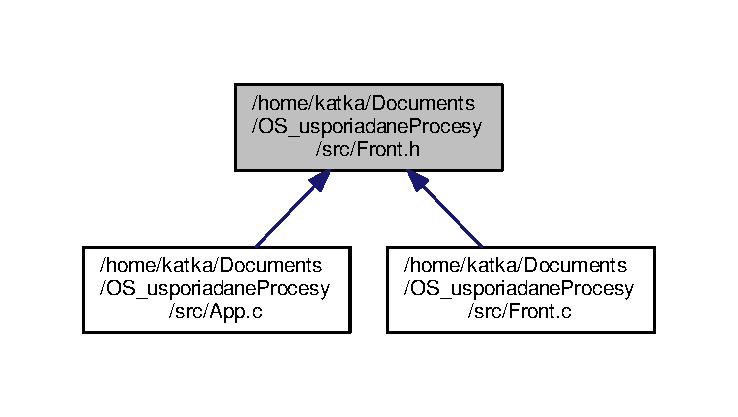
\includegraphics[width=350pt]{Front_8h__dep__incl}
\end{center}
\end{figure}
\subsection*{Classes}
\begin{DoxyCompactItemize}
\item 
struct \hyperlink{struct__Front}{\+\_\+\+Front}
\begin{DoxyCompactList}\small\item\em Pseudo-\/objekt specifikacia atributov. \end{DoxyCompactList}\end{DoxyCompactItemize}
\subsection*{Typedefs}
\begin{DoxyCompactItemize}
\item 
typedef struct \hyperlink{struct__Front}{\+\_\+\+Front} \hyperlink{Front_8h_aeda6f9a18e68a801590717ec948afc22}{Front}
\begin{DoxyCompactList}\small\item\em Pseudo-\/objekt specifikacia atributov. \end{DoxyCompactList}\end{DoxyCompactItemize}
\subsection*{Functions}
\begin{DoxyCompactItemize}
\item 
\hyperlink{Front_8h_aeda6f9a18e68a801590717ec948afc22}{Front} $\ast$ \hyperlink{Front_8h_a0c58eb9ce291fecc6b520a9a00130de8}{up\+\_\+front\+\_\+vytvor} ()
\begin{DoxyCompactList}\small\item\em Inicializuje front. \end{DoxyCompactList}\item 
void \hyperlink{Front_8h_aa5f6d4ff6866b68e7a82ab188d1e582d}{up\+\_\+front\+\_\+zrus} (\hyperlink{Front_8h_aeda6f9a18e68a801590717ec948afc22}{Front} $\ast$inst)
\begin{DoxyCompactList}\small\item\em Zrusenie frontu. \end{DoxyCompactList}\item 
void \hyperlink{Front_8h_ac80877645f112df1ece1c73b06f79a80}{up\+\_\+front\+\_\+push} (\hyperlink{Front_8h_aeda6f9a18e68a801590717ec948afc22}{Front} $\ast$inst, void $\ast$prvok)
\begin{DoxyCompactList}\small\item\em Pridanie prvku do frontu. \end{DoxyCompactList}\item 
void $\ast$ \hyperlink{Front_8h_ae43c9590e0c795e07914f0965aa917da}{up\+\_\+front\+\_\+pop} (\hyperlink{Front_8h_aeda6f9a18e68a801590717ec948afc22}{Front} $\ast$inst)
\begin{DoxyCompactList}\small\item\em Odobratie prvku z frontu. \end{DoxyCompactList}\item 
void $\ast$ \hyperlink{Front_8h_a23dea24023ffd88914ef499bf0d0c64c}{up\+\_\+front\+\_\+peek} (\hyperlink{Front_8h_aeda6f9a18e68a801590717ec948afc22}{Front} $\ast$inst)
\begin{DoxyCompactList}\small\item\em Spristupnenie prveho prvku na pop. \end{DoxyCompactList}\item 
int \hyperlink{Front_8h_a63e5753b29437dde3926a4b91ca344b1}{up\+\_\+front\+\_\+je\+\_\+prazdny} (\hyperlink{Front_8h_aeda6f9a18e68a801590717ec948afc22}{Front} $\ast$inst)
\begin{DoxyCompactList}\small\item\em Zisti, ci je front prazdny. \end{DoxyCompactList}\item 
size\+\_\+t \hyperlink{Front_8h_a92a54c47c61758146e7c9205f598938f}{up\+\_\+front\+\_\+daj\+\_\+poc\+\_\+prvkov} (\hyperlink{Front_8h_aeda6f9a18e68a801590717ec948afc22}{Front} $\ast$inst)
\begin{DoxyCompactList}\small\item\em Vrati pocet prvkov frontu. \end{DoxyCompactList}\end{DoxyCompactItemize}


\subsection{Detailed Description}
Modul zodpoveny za riadenie a vytvorenie udajovej strukury front. 

\begin{DoxyAuthor}{Author}
Katarina Pilarcikova $<$\href{mailto:ketrin.pilarcik@gmail.com}{\tt ketrin.\+pilarcik@gmail.\+com} 
\end{DoxyAuthor}
\begin{DoxyDate}{Date}
20 Dec 2016 
\end{DoxyDate}


\subsection{Typedef Documentation}
\index{Front.\+h@{Front.\+h}!Front@{Front}}
\index{Front@{Front}!Front.\+h@{Front.\+h}}
\subsubsection[{\texorpdfstring{Front}{Front}}]{\setlength{\rightskip}{0pt plus 5cm}typedef struct {\bf \+\_\+\+Front}  {\bf Front}}\hypertarget{Front_8h_aeda6f9a18e68a801590717ec948afc22}{}\label{Front_8h_aeda6f9a18e68a801590717ec948afc22}


Pseudo-\/objekt specifikacia atributov. 

Reprezentuje instanciu udajovej struktury front implementovany implicitne. 

\subsection{Function Documentation}
\index{Front.\+h@{Front.\+h}!up\+\_\+front\+\_\+daj\+\_\+poc\+\_\+prvkov@{up\+\_\+front\+\_\+daj\+\_\+poc\+\_\+prvkov}}
\index{up\+\_\+front\+\_\+daj\+\_\+poc\+\_\+prvkov@{up\+\_\+front\+\_\+daj\+\_\+poc\+\_\+prvkov}!Front.\+h@{Front.\+h}}
\subsubsection[{\texorpdfstring{up\+\_\+front\+\_\+daj\+\_\+poc\+\_\+prvkov(\+Front $\ast$inst)}{up_front_daj_poc_prvkov(Front *inst)}}]{\setlength{\rightskip}{0pt plus 5cm}size\+\_\+t up\+\_\+front\+\_\+daj\+\_\+poc\+\_\+prvkov (
\begin{DoxyParamCaption}
\item[{{\bf Front} $\ast$}]{inst}
\end{DoxyParamCaption}
)}\hypertarget{Front_8h_a92a54c47c61758146e7c9205f598938f}{}\label{Front_8h_a92a54c47c61758146e7c9205f598938f}


Vrati pocet prvkov frontu. 


\begin{DoxyParams}{Parameters}
{\em inst} & Instancia frontu \\
\hline
\end{DoxyParams}
\begin{DoxyReturn}{Returns}
size\+\_\+t Aktualny pocet prvkov frontu. 
\end{DoxyReturn}
\index{Front.\+h@{Front.\+h}!up\+\_\+front\+\_\+je\+\_\+prazdny@{up\+\_\+front\+\_\+je\+\_\+prazdny}}
\index{up\+\_\+front\+\_\+je\+\_\+prazdny@{up\+\_\+front\+\_\+je\+\_\+prazdny}!Front.\+h@{Front.\+h}}
\subsubsection[{\texorpdfstring{up\+\_\+front\+\_\+je\+\_\+prazdny(\+Front $\ast$inst)}{up_front_je_prazdny(Front *inst)}}]{\setlength{\rightskip}{0pt plus 5cm}int up\+\_\+front\+\_\+je\+\_\+prazdny (
\begin{DoxyParamCaption}
\item[{{\bf Front} $\ast$}]{inst}
\end{DoxyParamCaption}
)}\hypertarget{Front_8h_a63e5753b29437dde3926a4b91ca344b1}{}\label{Front_8h_a63e5753b29437dde3926a4b91ca344b1}


Zisti, ci je front prazdny. 


\begin{DoxyParams}{Parameters}
{\em inst} & Instancia frontu \\
\hline
\end{DoxyParams}
\begin{DoxyReturn}{Returns}
0 ak obsahuje prvky, 1 aj je prazdny. 
\end{DoxyReturn}
\index{Front.\+h@{Front.\+h}!up\+\_\+front\+\_\+peek@{up\+\_\+front\+\_\+peek}}
\index{up\+\_\+front\+\_\+peek@{up\+\_\+front\+\_\+peek}!Front.\+h@{Front.\+h}}
\subsubsection[{\texorpdfstring{up\+\_\+front\+\_\+peek(\+Front $\ast$inst)}{up_front_peek(Front *inst)}}]{\setlength{\rightskip}{0pt plus 5cm}void$\ast$ up\+\_\+front\+\_\+peek (
\begin{DoxyParamCaption}
\item[{{\bf Front} $\ast$}]{inst}
\end{DoxyParamCaption}
)}\hypertarget{Front_8h_a23dea24023ffd88914ef499bf0d0c64c}{}\label{Front_8h_a23dea24023ffd88914ef499bf0d0c64c}


Spristupnenie prveho prvku na pop. 


\begin{DoxyParams}{Parameters}
{\em inst} & Instancia frontu z ktoreho zistujeme prvok. \\
\hline
\end{DoxyParams}
\index{Front.\+h@{Front.\+h}!up\+\_\+front\+\_\+pop@{up\+\_\+front\+\_\+pop}}
\index{up\+\_\+front\+\_\+pop@{up\+\_\+front\+\_\+pop}!Front.\+h@{Front.\+h}}
\subsubsection[{\texorpdfstring{up\+\_\+front\+\_\+pop(\+Front $\ast$inst)}{up_front_pop(Front *inst)}}]{\setlength{\rightskip}{0pt plus 5cm}void$\ast$ up\+\_\+front\+\_\+pop (
\begin{DoxyParamCaption}
\item[{{\bf Front} $\ast$}]{inst}
\end{DoxyParamCaption}
)}\hypertarget{Front_8h_ae43c9590e0c795e07914f0965aa917da}{}\label{Front_8h_ae43c9590e0c795e07914f0965aa917da}


Odobratie prvku z frontu. 


\begin{DoxyParams}{Parameters}
{\em inst} & Instancia frontu z ktoreho vyberame. \\
\hline
\end{DoxyParams}
\begin{DoxyReturn}{Returns}
Prvok z prvy vo fronte. 
\end{DoxyReturn}
\index{Front.\+h@{Front.\+h}!up\+\_\+front\+\_\+push@{up\+\_\+front\+\_\+push}}
\index{up\+\_\+front\+\_\+push@{up\+\_\+front\+\_\+push}!Front.\+h@{Front.\+h}}
\subsubsection[{\texorpdfstring{up\+\_\+front\+\_\+push(\+Front $\ast$inst, void $\ast$prvok)}{up_front_push(Front *inst, void *prvok)}}]{\setlength{\rightskip}{0pt plus 5cm}void up\+\_\+front\+\_\+push (
\begin{DoxyParamCaption}
\item[{{\bf Front} $\ast$}]{inst, }
\item[{void $\ast$}]{prvok}
\end{DoxyParamCaption}
)}\hypertarget{Front_8h_ac80877645f112df1ece1c73b06f79a80}{}\label{Front_8h_ac80877645f112df1ece1c73b06f79a80}


Pridanie prvku do frontu. 


\begin{DoxyParams}{Parameters}
{\em inst} & Instancia frontu do ktoreho chceme pridat prvok. \\
\hline
{\em prvok} & Pridavany prvok do frontu. \\
\hline
\end{DoxyParams}
\index{Front.\+h@{Front.\+h}!up\+\_\+front\+\_\+vytvor@{up\+\_\+front\+\_\+vytvor}}
\index{up\+\_\+front\+\_\+vytvor@{up\+\_\+front\+\_\+vytvor}!Front.\+h@{Front.\+h}}
\subsubsection[{\texorpdfstring{up\+\_\+front\+\_\+vytvor()}{up_front_vytvor()}}]{\setlength{\rightskip}{0pt plus 5cm}{\bf Front}$\ast$ up\+\_\+front\+\_\+vytvor (
\begin{DoxyParamCaption}
{}
\end{DoxyParamCaption}
)}\hypertarget{Front_8h_a0c58eb9ce291fecc6b520a9a00130de8}{}\label{Front_8h_a0c58eb9ce291fecc6b520a9a00130de8}


Inicializuje front. 

\begin{DoxyReturn}{Returns}
Pointer na instanciu frontu 
\end{DoxyReturn}
\index{Front.\+h@{Front.\+h}!up\+\_\+front\+\_\+zrus@{up\+\_\+front\+\_\+zrus}}
\index{up\+\_\+front\+\_\+zrus@{up\+\_\+front\+\_\+zrus}!Front.\+h@{Front.\+h}}
\subsubsection[{\texorpdfstring{up\+\_\+front\+\_\+zrus(\+Front $\ast$inst)}{up_front_zrus(Front *inst)}}]{\setlength{\rightskip}{0pt plus 5cm}void up\+\_\+front\+\_\+zrus (
\begin{DoxyParamCaption}
\item[{{\bf Front} $\ast$}]{inst}
\end{DoxyParamCaption}
)}\hypertarget{Front_8h_aa5f6d4ff6866b68e7a82ab188d1e582d}{}\label{Front_8h_aa5f6d4ff6866b68e7a82ab188d1e582d}


Zrusenie frontu. 


\begin{DoxyParams}{Parameters}
{\em inst} & Smernik na instanciu frontu, kt pozadujeme zrusit. \\
\hline
\end{DoxyParams}

\hypertarget{Matica_8c}{}\section{/home/katka/\+Documents/\+O\+S\+\_\+usporiadane\+Procesy/src/\+Matica.c File Reference}
\label{Matica_8c}\index{/home/katka/\+Documents/\+O\+S\+\_\+usporiadane\+Procesy/src/\+Matica.\+c@{/home/katka/\+Documents/\+O\+S\+\_\+usporiadane\+Procesy/src/\+Matica.\+c}}


Modul zodpoveny za riadenie a vytvorenie incidencnej matice.  


{\ttfamily \#include $<$stdlib.\+h$>$}\\*
{\ttfamily \#include $<$stdio.\+h$>$}\\*
{\ttfamily \#include $<$string.\+h$>$}\\*
{\ttfamily \#include \char`\"{}Matica.\+h\char`\"{}}\\*
Include dependency graph for Matica.\+c\+:
\nopagebreak
\begin{figure}[H]
\begin{center}
\leavevmode
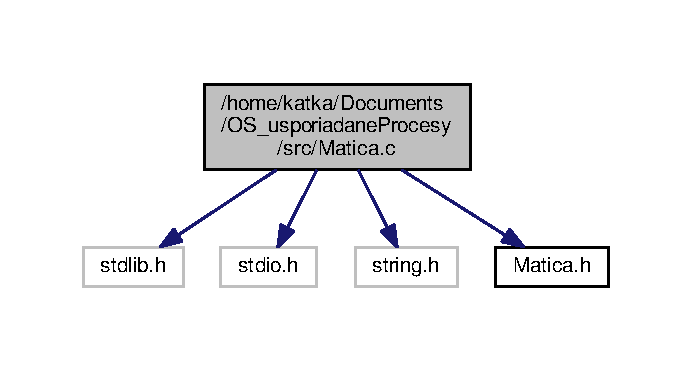
\includegraphics[width=332pt]{Matica_8c__incl}
\end{center}
\end{figure}
\subsection*{Functions}
\begin{DoxyCompactItemize}
\item 
\hyperlink{Matica_8h_a785a7a4c713ff8e23354dd49e33b1fef}{Matica} $\ast$ \hyperlink{Matica_8c_ada67edbf7d426d1e1fda7d379344ea27}{up\+\_\+matica\+\_\+vytvor} (size\+\_\+t velkost\+\_\+strany)
\begin{DoxyCompactList}\small\item\em Inicializacia matice. \end{DoxyCompactList}\item 
int $\ast$$\ast$ \hyperlink{Matica_8c_a2a2da1386f6c15a5d424ee4bd9750f66}{up\+\_\+matica\+\_\+vrat\+\_\+pole} (\hyperlink{Matica_8h_a785a7a4c713ff8e23354dd49e33b1fef}{Matica} $\ast$inst)
\begin{DoxyCompactList}\small\item\em Vrati pole matice. \end{DoxyCompactList}\item 
size\+\_\+t \hyperlink{Matica_8c_ac145e2dc659ccefbda6c2bb76cdd9030}{up\+\_\+matica\+\_\+daj\+\_\+velkost} (\hyperlink{Matica_8h_a785a7a4c713ff8e23354dd49e33b1fef}{Matica} $\ast$inst)
\begin{DoxyCompactList}\small\item\em Vrati velkost matice. \end{DoxyCompactList}\item 
void \hyperlink{Matica_8c_a36faa601f0d5f5defe12cc0ce6b27fe1}{up\+\_\+matica\+\_\+vypis} (\hyperlink{Matica_8h_a785a7a4c713ff8e23354dd49e33b1fef}{Matica} $\ast$inst)
\begin{DoxyCompactList}\small\item\em Vypise maticu na obrazovku. \end{DoxyCompactList}\item 
void \hyperlink{Matica_8c_aa122f233d1f23bf8c4a84ab54aef6d01}{up\+\_\+matica\+\_\+zrus} (\hyperlink{Matica_8h_a785a7a4c713ff8e23354dd49e33b1fef}{Matica} $\ast$inst)
\begin{DoxyCompactList}\small\item\em Zrusi maticu. \end{DoxyCompactList}\end{DoxyCompactItemize}


\subsection{Detailed Description}
Modul zodpoveny za riadenie a vytvorenie incidencnej matice. 

\begin{DoxyAuthor}{Author}
Katarina Pilarcikova $<$\href{mailto:ketrin.pilarcik@gmail.com}{\tt ketrin.\+pilarcik@gmail.\+com} 
\end{DoxyAuthor}
\begin{DoxyDate}{Date}
20 Dec 2016 
\end{DoxyDate}


\subsection{Function Documentation}
\index{Matica.\+c@{Matica.\+c}!up\+\_\+matica\+\_\+daj\+\_\+velkost@{up\+\_\+matica\+\_\+daj\+\_\+velkost}}
\index{up\+\_\+matica\+\_\+daj\+\_\+velkost@{up\+\_\+matica\+\_\+daj\+\_\+velkost}!Matica.\+c@{Matica.\+c}}
\subsubsection[{\texorpdfstring{up\+\_\+matica\+\_\+daj\+\_\+velkost(\+Matica $\ast$inst)}{up_matica_daj_velkost(Matica *inst)}}]{\setlength{\rightskip}{0pt plus 5cm}size\+\_\+t up\+\_\+matica\+\_\+daj\+\_\+velkost (
\begin{DoxyParamCaption}
\item[{{\bf Matica} $\ast$}]{inst}
\end{DoxyParamCaption}
)}\hypertarget{Matica_8c_ac145e2dc659ccefbda6c2bb76cdd9030}{}\label{Matica_8c_ac145e2dc659ccefbda6c2bb76cdd9030}


Vrati velkost matice. 


\begin{DoxyParams}{Parameters}
{\em inst} & Instancia matice. \\
\hline
\end{DoxyParams}
\begin{DoxyReturn}{Returns}
Velkost matice. 
\end{DoxyReturn}
\index{Matica.\+c@{Matica.\+c}!up\+\_\+matica\+\_\+vrat\+\_\+pole@{up\+\_\+matica\+\_\+vrat\+\_\+pole}}
\index{up\+\_\+matica\+\_\+vrat\+\_\+pole@{up\+\_\+matica\+\_\+vrat\+\_\+pole}!Matica.\+c@{Matica.\+c}}
\subsubsection[{\texorpdfstring{up\+\_\+matica\+\_\+vrat\+\_\+pole(\+Matica $\ast$inst)}{up_matica_vrat_pole(Matica *inst)}}]{\setlength{\rightskip}{0pt plus 5cm}int$\ast$$\ast$ up\+\_\+matica\+\_\+vrat\+\_\+pole (
\begin{DoxyParamCaption}
\item[{{\bf Matica} $\ast$}]{inst}
\end{DoxyParamCaption}
)}\hypertarget{Matica_8c_a2a2da1386f6c15a5d424ee4bd9750f66}{}\label{Matica_8c_a2a2da1386f6c15a5d424ee4bd9750f66}


Vrati pole matice. 


\begin{DoxyParams}{Parameters}
{\em inst} & Instancia matice. \\
\hline
\end{DoxyParams}
\begin{DoxyReturn}{Returns}
Pole matice. 
\end{DoxyReturn}
\index{Matica.\+c@{Matica.\+c}!up\+\_\+matica\+\_\+vypis@{up\+\_\+matica\+\_\+vypis}}
\index{up\+\_\+matica\+\_\+vypis@{up\+\_\+matica\+\_\+vypis}!Matica.\+c@{Matica.\+c}}
\subsubsection[{\texorpdfstring{up\+\_\+matica\+\_\+vypis(\+Matica $\ast$inst)}{up_matica_vypis(Matica *inst)}}]{\setlength{\rightskip}{0pt plus 5cm}void up\+\_\+matica\+\_\+vypis (
\begin{DoxyParamCaption}
\item[{{\bf Matica} $\ast$}]{inst}
\end{DoxyParamCaption}
)}\hypertarget{Matica_8c_a36faa601f0d5f5defe12cc0ce6b27fe1}{}\label{Matica_8c_a36faa601f0d5f5defe12cc0ce6b27fe1}


Vypise maticu na obrazovku. 


\begin{DoxyParams}{Parameters}
{\em inst} & Instancia matice. \\
\hline
\end{DoxyParams}
\index{Matica.\+c@{Matica.\+c}!up\+\_\+matica\+\_\+vytvor@{up\+\_\+matica\+\_\+vytvor}}
\index{up\+\_\+matica\+\_\+vytvor@{up\+\_\+matica\+\_\+vytvor}!Matica.\+c@{Matica.\+c}}
\subsubsection[{\texorpdfstring{up\+\_\+matica\+\_\+vytvor(size\+\_\+t velkost\+\_\+strany)}{up_matica_vytvor(size_t velkost_strany)}}]{\setlength{\rightskip}{0pt plus 5cm}{\bf Matica}$\ast$ up\+\_\+matica\+\_\+vytvor (
\begin{DoxyParamCaption}
\item[{size\+\_\+t}]{velkost\+\_\+strany}
\end{DoxyParamCaption}
)}\hypertarget{Matica_8c_ada67edbf7d426d1e1fda7d379344ea27}{}\label{Matica_8c_ada67edbf7d426d1e1fda7d379344ea27}


Inicializacia matice. 


\begin{DoxyParams}{Parameters}
{\em velkost\+\_\+strany} & Velkost strany matice, s ktorou ma byt vytvorena. \\
\hline
\end{DoxyParams}
\begin{DoxyReturn}{Returns}
Instancia matice. 
\end{DoxyReturn}
\index{Matica.\+c@{Matica.\+c}!up\+\_\+matica\+\_\+zrus@{up\+\_\+matica\+\_\+zrus}}
\index{up\+\_\+matica\+\_\+zrus@{up\+\_\+matica\+\_\+zrus}!Matica.\+c@{Matica.\+c}}
\subsubsection[{\texorpdfstring{up\+\_\+matica\+\_\+zrus(\+Matica $\ast$inst)}{up_matica_zrus(Matica *inst)}}]{\setlength{\rightskip}{0pt plus 5cm}void up\+\_\+matica\+\_\+zrus (
\begin{DoxyParamCaption}
\item[{{\bf Matica} $\ast$}]{inst}
\end{DoxyParamCaption}
)}\hypertarget{Matica_8c_aa122f233d1f23bf8c4a84ab54aef6d01}{}\label{Matica_8c_aa122f233d1f23bf8c4a84ab54aef6d01}


Zrusi maticu. 


\begin{DoxyParams}{Parameters}
{\em inst} & Instancia matice. \\
\hline
\end{DoxyParams}

\hypertarget{Matica_8h}{}\section{/home/katka/\+Documents/\+O\+S\+\_\+usporiadane\+Procesy/src/\+Matica.h File Reference}
\label{Matica_8h}\index{/home/katka/\+Documents/\+O\+S\+\_\+usporiadane\+Procesy/src/\+Matica.\+h@{/home/katka/\+Documents/\+O\+S\+\_\+usporiadane\+Procesy/src/\+Matica.\+h}}


Modul zodpoveny za riadenie a vytvorenie incidencnej matice.  


This graph shows which files directly or indirectly include this file\+:
\nopagebreak
\begin{figure}[H]
\begin{center}
\leavevmode
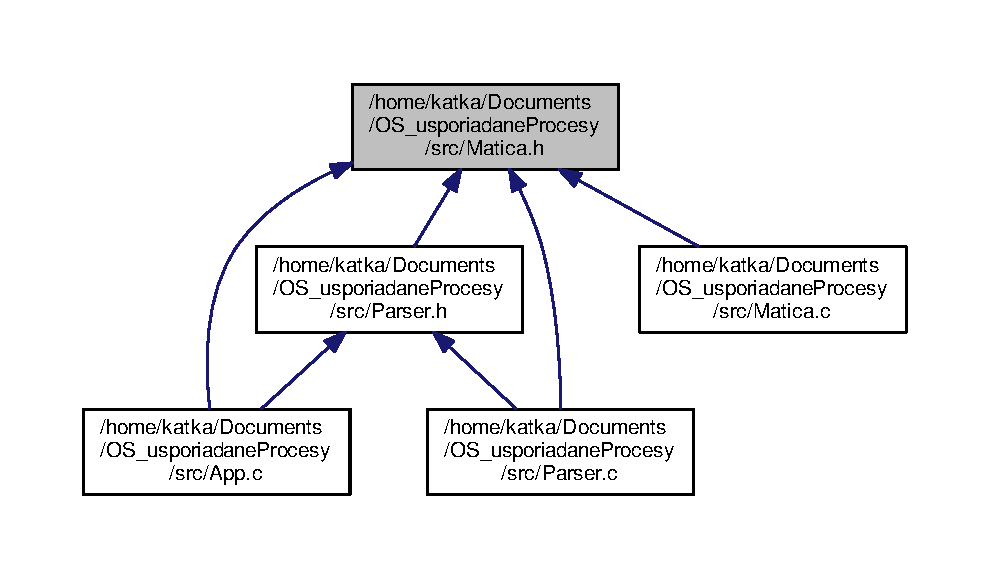
\includegraphics[width=350pt]{Matica_8h__dep__incl}
\end{center}
\end{figure}
\subsection*{Classes}
\begin{DoxyCompactItemize}
\item 
struct \hyperlink{struct__Matica}{\+\_\+\+Matica}
\begin{DoxyCompactList}\small\item\em Pseudo-\/objekt specifikuje atributy. \end{DoxyCompactList}\end{DoxyCompactItemize}
\subsection*{Typedefs}
\begin{DoxyCompactItemize}
\item 
typedef struct \hyperlink{struct__Matica}{\+\_\+\+Matica} \hyperlink{Matica_8h_a785a7a4c713ff8e23354dd49e33b1fef}{Matica}
\begin{DoxyCompactList}\small\item\em Pseudo-\/objekt specifikuje atributy. \end{DoxyCompactList}\end{DoxyCompactItemize}
\subsection*{Functions}
\begin{DoxyCompactItemize}
\item 
\hyperlink{Matica_8h_a785a7a4c713ff8e23354dd49e33b1fef}{Matica} $\ast$ \hyperlink{Matica_8h_ada67edbf7d426d1e1fda7d379344ea27}{up\+\_\+matica\+\_\+vytvor} (size\+\_\+t velkost\+\_\+strany)
\begin{DoxyCompactList}\small\item\em Inicializacia matice. \end{DoxyCompactList}\item 
int $\ast$$\ast$ \hyperlink{Matica_8h_a2a2da1386f6c15a5d424ee4bd9750f66}{up\+\_\+matica\+\_\+vrat\+\_\+pole} (\hyperlink{Matica_8h_a785a7a4c713ff8e23354dd49e33b1fef}{Matica} $\ast$inst)
\begin{DoxyCompactList}\small\item\em Vrati pole matice. \end{DoxyCompactList}\item 
size\+\_\+t \hyperlink{Matica_8h_ac145e2dc659ccefbda6c2bb76cdd9030}{up\+\_\+matica\+\_\+daj\+\_\+velkost} (\hyperlink{Matica_8h_a785a7a4c713ff8e23354dd49e33b1fef}{Matica} $\ast$inst)
\begin{DoxyCompactList}\small\item\em Vrati velkost matice. \end{DoxyCompactList}\item 
void \hyperlink{Matica_8h_a36faa601f0d5f5defe12cc0ce6b27fe1}{up\+\_\+matica\+\_\+vypis} (\hyperlink{Matica_8h_a785a7a4c713ff8e23354dd49e33b1fef}{Matica} $\ast$inst)
\begin{DoxyCompactList}\small\item\em Vypise maticu na obrazovku. \end{DoxyCompactList}\item 
void \hyperlink{Matica_8h_aa122f233d1f23bf8c4a84ab54aef6d01}{up\+\_\+matica\+\_\+zrus} (\hyperlink{Matica_8h_a785a7a4c713ff8e23354dd49e33b1fef}{Matica} $\ast$inst)
\begin{DoxyCompactList}\small\item\em Zrusi maticu. \end{DoxyCompactList}\end{DoxyCompactItemize}


\subsection{Detailed Description}
Modul zodpoveny za riadenie a vytvorenie incidencnej matice. 

\begin{DoxyAuthor}{Author}
Katarina Pilarcikova $<$\href{mailto:ketrin.pilarcik@gmail.com}{\tt ketrin.\+pilarcik@gmail.\+com} 
\end{DoxyAuthor}
\begin{DoxyDate}{Date}
20 Dec 2016 
\end{DoxyDate}


\subsection{Typedef Documentation}
\index{Matica.\+h@{Matica.\+h}!Matica@{Matica}}
\index{Matica@{Matica}!Matica.\+h@{Matica.\+h}}
\subsubsection[{\texorpdfstring{Matica}{Matica}}]{\setlength{\rightskip}{0pt plus 5cm}typedef struct {\bf \+\_\+\+Matica}  {\bf Matica}}\hypertarget{Matica_8h_a785a7a4c713ff8e23354dd49e33b1fef}{}\label{Matica_8h_a785a7a4c713ff8e23354dd49e33b1fef}


Pseudo-\/objekt specifikuje atributy. 

Reprezentuje instanciu matice. 

\subsection{Function Documentation}
\index{Matica.\+h@{Matica.\+h}!up\+\_\+matica\+\_\+daj\+\_\+velkost@{up\+\_\+matica\+\_\+daj\+\_\+velkost}}
\index{up\+\_\+matica\+\_\+daj\+\_\+velkost@{up\+\_\+matica\+\_\+daj\+\_\+velkost}!Matica.\+h@{Matica.\+h}}
\subsubsection[{\texorpdfstring{up\+\_\+matica\+\_\+daj\+\_\+velkost(\+Matica $\ast$inst)}{up_matica_daj_velkost(Matica *inst)}}]{\setlength{\rightskip}{0pt plus 5cm}size\+\_\+t up\+\_\+matica\+\_\+daj\+\_\+velkost (
\begin{DoxyParamCaption}
\item[{{\bf Matica} $\ast$}]{inst}
\end{DoxyParamCaption}
)}\hypertarget{Matica_8h_ac145e2dc659ccefbda6c2bb76cdd9030}{}\label{Matica_8h_ac145e2dc659ccefbda6c2bb76cdd9030}


Vrati velkost matice. 


\begin{DoxyParams}{Parameters}
{\em inst} & Instancia matice. \\
\hline
\end{DoxyParams}
\begin{DoxyReturn}{Returns}
Velkost matice. 
\end{DoxyReturn}
\index{Matica.\+h@{Matica.\+h}!up\+\_\+matica\+\_\+vrat\+\_\+pole@{up\+\_\+matica\+\_\+vrat\+\_\+pole}}
\index{up\+\_\+matica\+\_\+vrat\+\_\+pole@{up\+\_\+matica\+\_\+vrat\+\_\+pole}!Matica.\+h@{Matica.\+h}}
\subsubsection[{\texorpdfstring{up\+\_\+matica\+\_\+vrat\+\_\+pole(\+Matica $\ast$inst)}{up_matica_vrat_pole(Matica *inst)}}]{\setlength{\rightskip}{0pt plus 5cm}int$\ast$$\ast$ up\+\_\+matica\+\_\+vrat\+\_\+pole (
\begin{DoxyParamCaption}
\item[{{\bf Matica} $\ast$}]{inst}
\end{DoxyParamCaption}
)}\hypertarget{Matica_8h_a2a2da1386f6c15a5d424ee4bd9750f66}{}\label{Matica_8h_a2a2da1386f6c15a5d424ee4bd9750f66}


Vrati pole matice. 


\begin{DoxyParams}{Parameters}
{\em inst} & Instancia matice. \\
\hline
\end{DoxyParams}
\begin{DoxyReturn}{Returns}
Pole matice. 
\end{DoxyReturn}
\index{Matica.\+h@{Matica.\+h}!up\+\_\+matica\+\_\+vypis@{up\+\_\+matica\+\_\+vypis}}
\index{up\+\_\+matica\+\_\+vypis@{up\+\_\+matica\+\_\+vypis}!Matica.\+h@{Matica.\+h}}
\subsubsection[{\texorpdfstring{up\+\_\+matica\+\_\+vypis(\+Matica $\ast$inst)}{up_matica_vypis(Matica *inst)}}]{\setlength{\rightskip}{0pt plus 5cm}void up\+\_\+matica\+\_\+vypis (
\begin{DoxyParamCaption}
\item[{{\bf Matica} $\ast$}]{inst}
\end{DoxyParamCaption}
)}\hypertarget{Matica_8h_a36faa601f0d5f5defe12cc0ce6b27fe1}{}\label{Matica_8h_a36faa601f0d5f5defe12cc0ce6b27fe1}


Vypise maticu na obrazovku. 


\begin{DoxyParams}{Parameters}
{\em inst} & Instancia matice. \\
\hline
\end{DoxyParams}
\index{Matica.\+h@{Matica.\+h}!up\+\_\+matica\+\_\+vytvor@{up\+\_\+matica\+\_\+vytvor}}
\index{up\+\_\+matica\+\_\+vytvor@{up\+\_\+matica\+\_\+vytvor}!Matica.\+h@{Matica.\+h}}
\subsubsection[{\texorpdfstring{up\+\_\+matica\+\_\+vytvor(size\+\_\+t velkost\+\_\+strany)}{up_matica_vytvor(size_t velkost_strany)}}]{\setlength{\rightskip}{0pt plus 5cm}{\bf Matica}$\ast$ up\+\_\+matica\+\_\+vytvor (
\begin{DoxyParamCaption}
\item[{size\+\_\+t}]{velkost\+\_\+strany}
\end{DoxyParamCaption}
)}\hypertarget{Matica_8h_ada67edbf7d426d1e1fda7d379344ea27}{}\label{Matica_8h_ada67edbf7d426d1e1fda7d379344ea27}


Inicializacia matice. 


\begin{DoxyParams}{Parameters}
{\em velkost\+\_\+strany} & Velkost strany matice, s ktorou ma byt vytvorena. \\
\hline
\end{DoxyParams}
\begin{DoxyReturn}{Returns}
Instancia matice. 
\end{DoxyReturn}
\index{Matica.\+h@{Matica.\+h}!up\+\_\+matica\+\_\+zrus@{up\+\_\+matica\+\_\+zrus}}
\index{up\+\_\+matica\+\_\+zrus@{up\+\_\+matica\+\_\+zrus}!Matica.\+h@{Matica.\+h}}
\subsubsection[{\texorpdfstring{up\+\_\+matica\+\_\+zrus(\+Matica $\ast$inst)}{up_matica_zrus(Matica *inst)}}]{\setlength{\rightskip}{0pt plus 5cm}void up\+\_\+matica\+\_\+zrus (
\begin{DoxyParamCaption}
\item[{{\bf Matica} $\ast$}]{inst}
\end{DoxyParamCaption}
)}\hypertarget{Matica_8h_aa122f233d1f23bf8c4a84ab54aef6d01}{}\label{Matica_8h_aa122f233d1f23bf8c4a84ab54aef6d01}


Zrusi maticu. 


\begin{DoxyParams}{Parameters}
{\em inst} & Instancia matice. \\
\hline
\end{DoxyParams}

\hypertarget{Parser_8c}{}\section{/home/katka/\+Documents/\+O\+S\+\_\+usporiadane\+Procesy/src/\+Parser.c File Reference}
\label{Parser_8c}\index{/home/katka/\+Documents/\+O\+S\+\_\+usporiadane\+Procesy/src/\+Parser.\+c@{/home/katka/\+Documents/\+O\+S\+\_\+usporiadane\+Procesy/src/\+Parser.\+c}}


Modul zodpoveny za riadenie a vytvorenie incidencnej matice.  


{\ttfamily \#include $<$stdio.\+h$>$}\\*
{\ttfamily \#include $<$ctype.\+h$>$}\\*
{\ttfamily \#include $<$errno.\+h$>$}\\*
{\ttfamily \#include $<$stdlib.\+h$>$}\\*
{\ttfamily \#include $<$string.\+h$>$}\\*
{\ttfamily \#include \char`\"{}Matica.\+h\char`\"{}}\\*
{\ttfamily \#include \char`\"{}Parser.\+h\char`\"{}}\\*
Include dependency graph for Parser.\+c\+:
\nopagebreak
\begin{figure}[H]
\begin{center}
\leavevmode
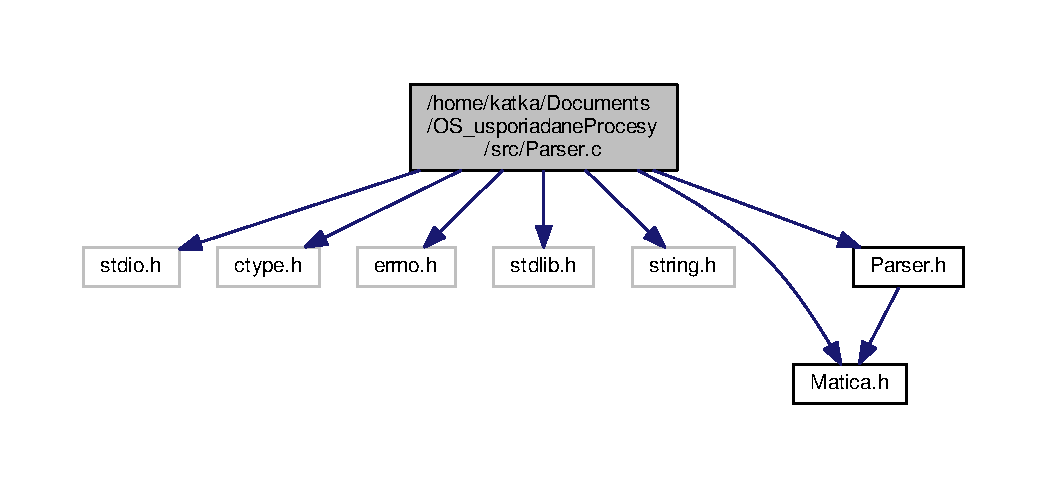
\includegraphics[width=350pt]{Parser_8c__incl}
\end{center}
\end{figure}
\subsection*{Macros}
\begin{DoxyCompactItemize}
\item 
\#define {\bfseries M\+A\+X\+\_\+\+P\+O\+C\+E\+T\+\_\+\+R\+I\+A\+D\+K\+OV}~3\hypertarget{Parser_8c_a2a907cd840b139cc1c5094b866e2417b}{}\label{Parser_8c_a2a907cd840b139cc1c5094b866e2417b}

\item 
\#define {\bfseries M\+A\+X\+\_\+\+D\+L\+Z\+K\+A\+\_\+\+R\+I\+A\+D\+KU}~50\hypertarget{Parser_8c_a3113fa2be67b23919e0b59dd45f1b3c4}{}\label{Parser_8c_a3113fa2be67b23919e0b59dd45f1b3c4}

\item 
\#define {\bfseries Z\+N\+A\+K\+\_\+\+N\+A\+\_\+\+C\+I\+S\+LO}(z)~((z) -\/ \textquotesingle{}0\textquotesingle{})\hypertarget{Parser_8c_a920b2ae9d7814a696f0edb31b126e276}{}\label{Parser_8c_a920b2ae9d7814a696f0edb31b126e276}

\end{DoxyCompactItemize}
\subsection*{Functions}
\begin{DoxyCompactItemize}
\item 
\hyperlink{Matica_8h_a785a7a4c713ff8e23354dd49e33b1fef}{Matica} $\ast$ \hyperlink{Parser_8c_a0149f861c9d51481d09195aa78ef3f5f}{up\+\_\+parser\+\_\+nacitaj\+\_\+subor} (const char $\ast$nazov\+\_\+suboru)
\begin{DoxyCompactList}\small\item\em Nacita vstupny subor orientovaneho grafu, spracuje a vytvori incidencnu maticu. \end{DoxyCompactList}\end{DoxyCompactItemize}


\subsection{Detailed Description}
Modul zodpoveny za riadenie a vytvorenie incidencnej matice. 

\begin{DoxyAuthor}{Author}
Katarina Pilarcikova $<$\href{mailto:ketrin.pilarcik@gmail.com}{\tt ketrin.\+pilarcik@gmail.\+com} 
\end{DoxyAuthor}
\begin{DoxyDate}{Date}
20 Dec 2016 
\end{DoxyDate}


\subsection{Function Documentation}
\index{Parser.\+c@{Parser.\+c}!up\+\_\+parser\+\_\+nacitaj\+\_\+subor@{up\+\_\+parser\+\_\+nacitaj\+\_\+subor}}
\index{up\+\_\+parser\+\_\+nacitaj\+\_\+subor@{up\+\_\+parser\+\_\+nacitaj\+\_\+subor}!Parser.\+c@{Parser.\+c}}
\subsubsection[{\texorpdfstring{up\+\_\+parser\+\_\+nacitaj\+\_\+subor(const char $\ast$nazov\+\_\+suboru)}{up_parser_nacitaj_subor(const char *nazov_suboru)}}]{\setlength{\rightskip}{0pt plus 5cm}{\bf Matica}$\ast$ up\+\_\+parser\+\_\+nacitaj\+\_\+subor (
\begin{DoxyParamCaption}
\item[{const char $\ast$}]{nazov\+\_\+suboru}
\end{DoxyParamCaption}
)}\hypertarget{Parser_8c_a0149f861c9d51481d09195aa78ef3f5f}{}\label{Parser_8c_a0149f861c9d51481d09195aa78ef3f5f}


Nacita vstupny subor orientovaneho grafu, spracuje a vytvori incidencnu maticu. 


\begin{DoxyParams}{Parameters}
{\em nazov\+\_\+suboru} & Nazov vstupneho suboru s orientovanym grafom. \\
\hline
\end{DoxyParams}
\begin{DoxyReturn}{Returns}
Instancia matice. 
\end{DoxyReturn}

\hypertarget{Parser_8h}{}\section{/home/katka/\+Documents/\+O\+S\+\_\+usporiadane\+Procesy/src/\+Parser.h File Reference}
\label{Parser_8h}\index{/home/katka/\+Documents/\+O\+S\+\_\+usporiadane\+Procesy/src/\+Parser.\+h@{/home/katka/\+Documents/\+O\+S\+\_\+usporiadane\+Procesy/src/\+Parser.\+h}}


Modul zodpoveny za riadenie a vytvorenie incidencnej matice.  


{\ttfamily \#include \char`\"{}Matica.\+h\char`\"{}}\\*
Include dependency graph for Parser.\+h\+:\nopagebreak
\begin{figure}[H]
\begin{center}
\leavevmode
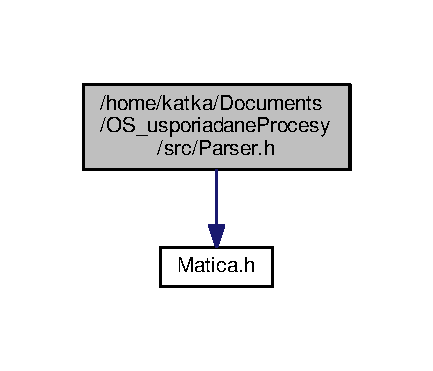
\includegraphics[width=208pt]{Parser_8h__incl}
\end{center}
\end{figure}
This graph shows which files directly or indirectly include this file\+:
\nopagebreak
\begin{figure}[H]
\begin{center}
\leavevmode
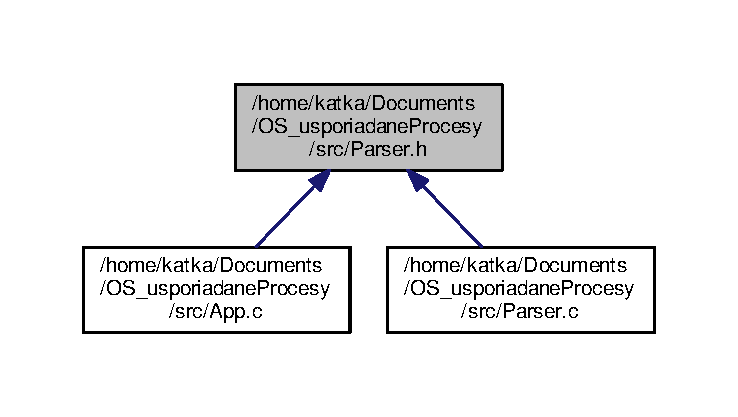
\includegraphics[width=350pt]{Parser_8h__dep__incl}
\end{center}
\end{figure}
\subsection*{Functions}
\begin{DoxyCompactItemize}
\item 
\hyperlink{Matica_8h_a785a7a4c713ff8e23354dd49e33b1fef}{Matica} $\ast$ \hyperlink{Parser_8h_a0149f861c9d51481d09195aa78ef3f5f}{up\+\_\+parser\+\_\+nacitaj\+\_\+subor} (const char $\ast$nazov\+\_\+suboru)
\begin{DoxyCompactList}\small\item\em Nacita vstupny subor orientovaneho grafu, spracuje a vytvori incidencnu maticu. \end{DoxyCompactList}\end{DoxyCompactItemize}


\subsection{Detailed Description}
Modul zodpoveny za riadenie a vytvorenie incidencnej matice. 

\begin{DoxyAuthor}{Author}
Katarina Pilarcikova $<$\href{mailto:ketrin.pilarcik@gmail.com}{\tt ketrin.\+pilarcik@gmail.\+com} 
\end{DoxyAuthor}
\begin{DoxyDate}{Date}
20 Dec 2016 
\end{DoxyDate}


\subsection{Function Documentation}
\index{Parser.\+h@{Parser.\+h}!up\+\_\+parser\+\_\+nacitaj\+\_\+subor@{up\+\_\+parser\+\_\+nacitaj\+\_\+subor}}
\index{up\+\_\+parser\+\_\+nacitaj\+\_\+subor@{up\+\_\+parser\+\_\+nacitaj\+\_\+subor}!Parser.\+h@{Parser.\+h}}
\subsubsection[{\texorpdfstring{up\+\_\+parser\+\_\+nacitaj\+\_\+subor(const char $\ast$nazov\+\_\+suboru)}{up_parser_nacitaj_subor(const char *nazov_suboru)}}]{\setlength{\rightskip}{0pt plus 5cm}{\bf Matica}$\ast$ up\+\_\+parser\+\_\+nacitaj\+\_\+subor (
\begin{DoxyParamCaption}
\item[{const char $\ast$}]{nazov\+\_\+suboru}
\end{DoxyParamCaption}
)}\hypertarget{Parser_8h_a0149f861c9d51481d09195aa78ef3f5f}{}\label{Parser_8h_a0149f861c9d51481d09195aa78ef3f5f}


Nacita vstupny subor orientovaneho grafu, spracuje a vytvori incidencnu maticu. 


\begin{DoxyParams}{Parameters}
{\em nazov\+\_\+suboru} & Nazov vstupneho suboru s orientovanym grafom. \\
\hline
\end{DoxyParams}
\begin{DoxyReturn}{Returns}
Instancia matice. 
\end{DoxyReturn}

%--- End generated contents ---

% Index
\backmatter
\newpage
\phantomsection
\clearemptydoublepage
\addcontentsline{toc}{chapter}{Index}
\printindex

\end{document}
